\section*{\nr.3 \titthree (25 Punkte)}
\begin{enumerate}[(a)]
\item Es gilt $E_0 = \hbar\omega/2$ und $E_3=7\hbar\omega/2$, also folgt:
\begin{equation}
E_0 = \frac{E_3}{7} = \frac{1}{7} \cdot \left(h c \cdot\SI{e4}{\per\centi\meter}\right) \approx \SI{0.18}{\electronvolt}
\end{equation}

\item 
\begin{equation}
E_3=\frac{7}{2}\hbar\omega \implies \omega = \frac{2E_3}{7\hbar} \approx \SI{5.39e14}{\hertz}
\end{equation}

\item Die Federkonstante $k$ berechnet sich zu:
\begin{equation}
k = m \omega^2 \approx \SI{4.81e2}{\newton\per\meter}
\end{equation}
Als Masse $m$ wurde die Masse des Wasserstoffkerns angesetzt, die hauptsächlich schwingt im Vergleich zum wesentlichen schwereren Chlor-Kern.
\item Eine Abbildung des genähert harmonischen Potentials mit den vier untersten Energieniveaus und den dazugehörigen Wellenfunktionen ist durch \vref{fig:potential} gegeben.
\begin{figure}[htbp]
\centering
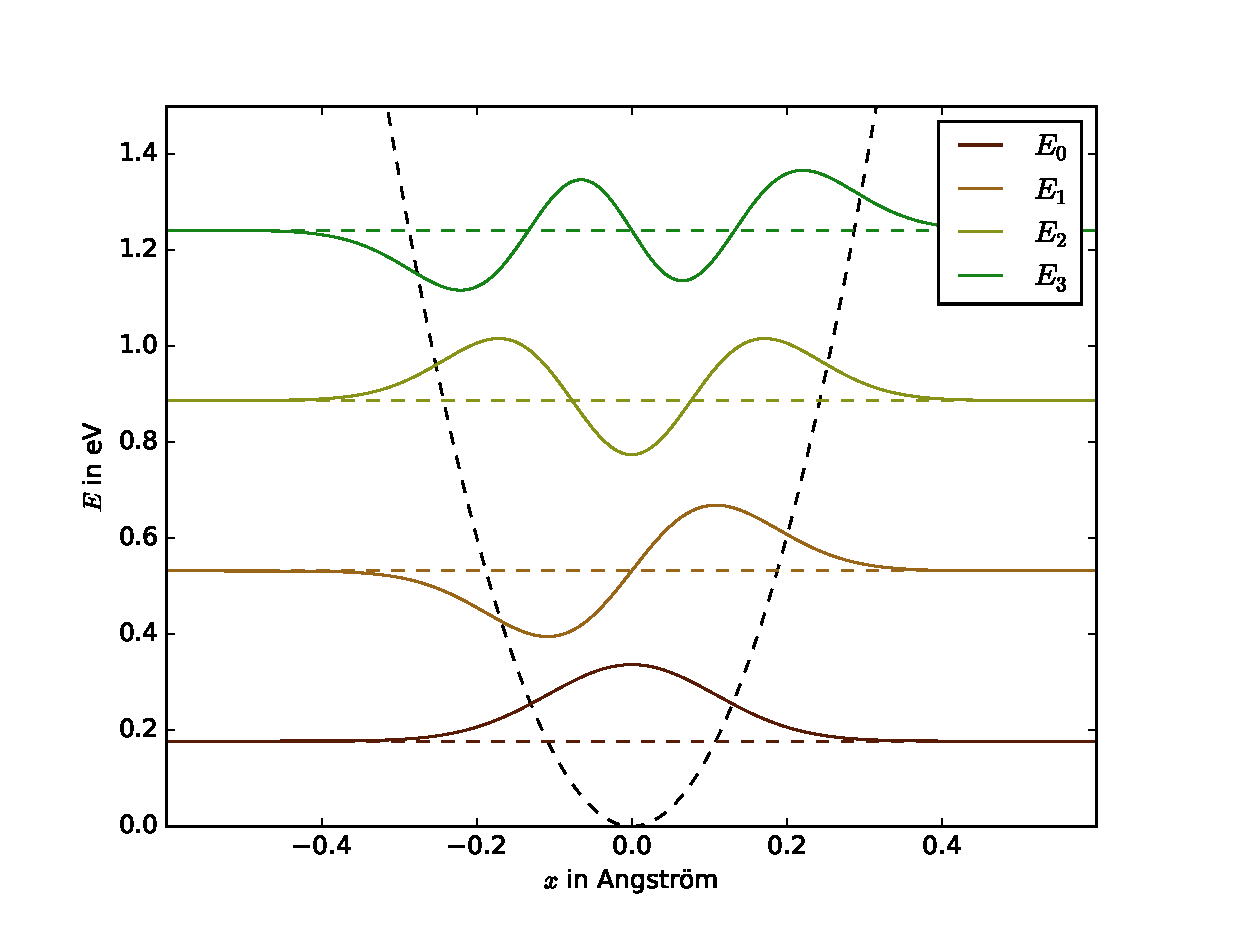
\includegraphics[width=\textwidth]{harmonic_potential.eps}
\caption{Die untersten vier Energiezustände des quantenharmonischen Oszillators mit den dazugehörigen Wellenfunktionen mit den Zahlenwerten der Aufgabe -- ein Wasserstoff-Atom im quadratischen Potential. Wellenfunktionen sind beliebig skaliert und auf das entsprechende Energieniveau verschoben.}
\label{fig:potential}
\end{figure}
\end{enumerate}